\chapter{Methods and Experiments} \label{methods-and-experiments}

\section{Single-Agent Bilateral Negotiation Environment (\gls{sbe})}
In this environment, the agent is a negotiator in a negotiation mechanism.

\subsection{Independent Negotiator in NegMAS}
SBE has just single learnable \gls{drl} negotiator. All RL algorithms with the correct type of action space and observation space can be tested in this specific environment. In the experiment of this thesis, some algorithms, such as DQN, PPO, A2C, from stable-baselines \ref{backgrounds:stable-baselines} are tested in four learning cases:
\begin{itemize}
	\item single issue, acceptance strategy
	\item single issue, offer strategy
	\item multi-issues, acceptance strategy
	\item multi-issues, offer startegy
\end{itemize}

The training logic of DQN is shown in the figure \ref{fig:dqn}, and the detailed description of this algorithm is shown in the appendix \ref{appendix:dqn}.

\begin{figure}[htbp]
\centering
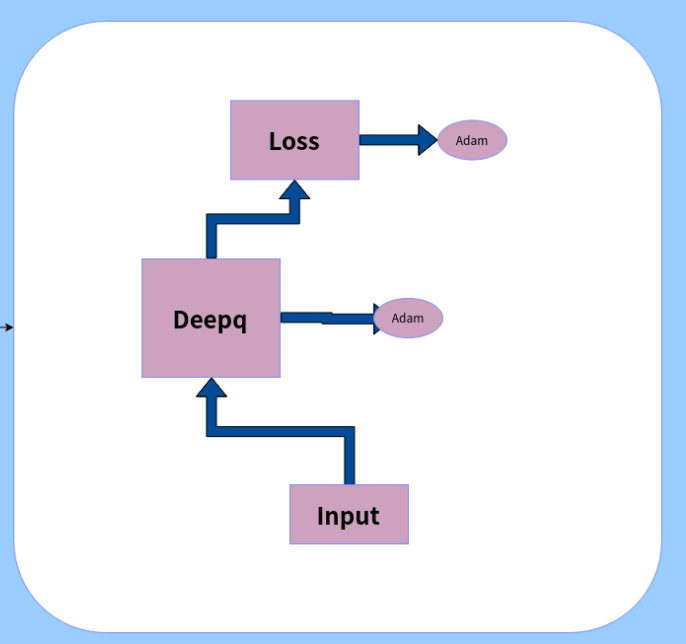
\includegraphics[width=0.30\textwidth]{./images/dqn.png}
\caption{Training logic of DQN}
\label{fig:dqn}
\end{figure}

\subsection{Experiment} \label{sbe:experiment}
Figure \ref{fig:bilateral-negotiation} depicts a game composed of two negotiators: \textbf{RL negotiator} and \textbf{Opponent negotiator} (AspirationNegotiator). The type of opponent negotiator can be changed in the settings file. All negotiators, which inherit the base abstract negotiator class in \gls{negmas} can be configured in the experiment. AspirationNegotiator is selected as the baseline negotiator in this experiment.

\begin{figure}[htbp]
\centering
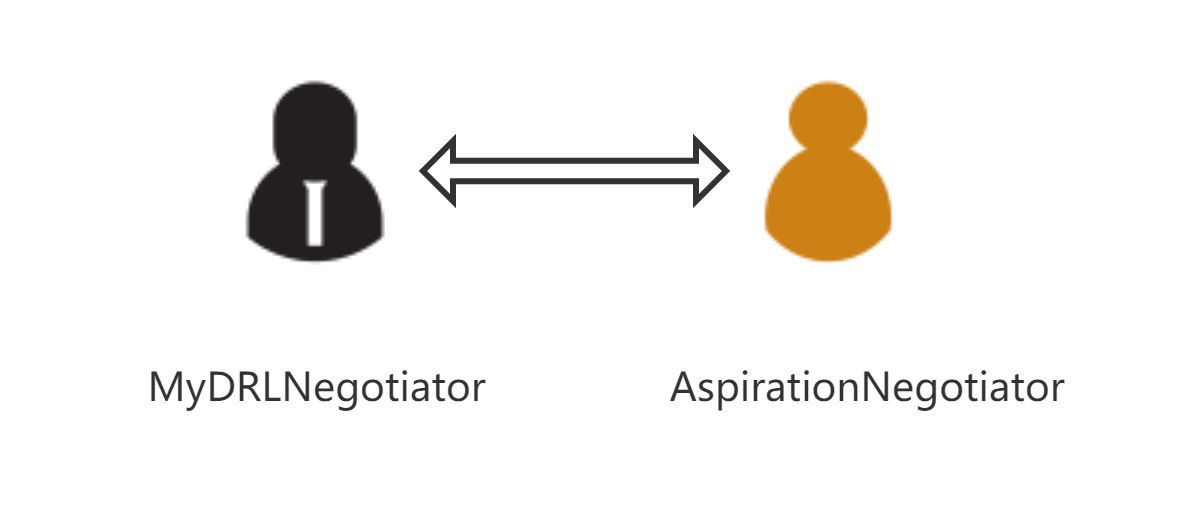
\includegraphics[width=0.50\textwidth]{./images/bilateral-negotiation.png}
\caption{Bilateral Negotiation Game in \gls{sbe}, My Deep Reinforcement Learning Negotiator vs. Aspiration Negotiator}
\label{fig:bilateral-negotiation}
\end{figure}

The negotiation mechanism is \gls{saom}, the RL negotiator can learn two strategies called \textbf{acceptance strategy} and \textbf{offer strategy}, which will be described in detail in the following paragraphs. 

\paragraph{Acceptance strategy} The variables observed by the agent are current offer of opponent and current time (running time, or relative round of negotiation mechanism).

\paragraph{Offer strategy} Actions of the negotiator are the set of outcomes in the outcome space. The observation space is the same as in the acceptance strategy. There is a special requirement when learning this strategy: Before feeding variables into the algorithm, observation is normalized. The equation of normalization is defined as follows:
\begin{equation}
\begin{aligned}
o^{\prime} = (rng_{max} - rng_{min}) \frac{o - o_{min}}{o_{max} - o_{min}} + rng_{min}
\end{aligned}
\end{equation}

Where $rng_{max}$ (1) and $rng_{min}$ (-1) are the boundary value of normalization. $o_{min}$ and $o_{max}$ represent the boundary value of the observation value. $o^{\prime}$ and $o$ are the normalized observation value and original observation value, respectively. 

Two different categories of agents are used for the experiments.

\paragraph{RL agent} was trained in the training environment for acceptance strategy and for offer strategy. Each strategy was learned under single issue (Table \ref{tab:attributes-sbe}) and under multi-issues (Table \ref{tab:attributes-sbe-multi-issues}) cases. 

\paragraph{Heuristic agents (e.g., AspirationNegotiator)} Negotiators were implemented in the package scml. In this experiment, the baseline negotiator is \textbf{ApsirationNegotiator} \ref{related-work:heuristic-negotiation}, which is a time-based heuristic negotiator.

\subsubsection{single issue}
The training environment is based on the \gls{sbe} and sets concrete limits and attributes for it, which are defined in table \ref{tab:attributes-sbe}.

\begin{table}[htbp]
\centering
\begin{tabular}{l l l} \toprule
\bfseries \textbf{Attributes}      & \bfseries \textbf{Value}             \\ \midrule
\textbf{Name}                    & negotiation\_env\_ac\_s, negotiation\_env\_of\_s \\
\textbf{Negotiation Mechanism}   & SAOMechanism                                        \\
\textbf{Max\_Steps}              & 100                                                 \\
\textbf{Issue}             	     & Price(300, 550)                                     \\
\textbf{Competitors}             & [MyDRLNegotiator, AspirationNegotiator]             \\
\textbf{Utility Functions}       & [LinearUtility(-0.35), LinearUtility(0.25)]         \\
\textbf{Actions}                 & [ACCEPT, REJCT, END, NO RESPONSE], Outcomes\\
\bottomrule
\end{tabular}
\caption{Attributes of the training environment (sbe), single-issue}
\label{tab:attributes-sbe}
\end{table}

Algorithms \gls{dqn}, \gls{ppo}, ACER\parencite{DBLP:journals/corr/WangBHMMKF16}, A2C and DDPG are tested in the case of single issue. The mean episode reward of all algorithms for \textbf{single issue, acceptance strategy} and \textbf{single issue, offer strategy} are shown in \ref{fig:single-issue}. \gls{dqn}, ACER, \gls{ppo} and A2C support discrete action space. Hence, these algorithms are used for training acceptance strategy, its action space is discrete. Additionally, \gls{ddpg}, \gls{ppo} and A2C can be used for training offer strategy, its action spaces can be considered as continuous. Mean episode reward is represented in two forms: 
\begin{itemize}
\item step: combines mean episode reward of all algorithms into one diagram.
\item wall: splits the mean episode reward of all algorithms as horizontal independente diagram.
\end{itemize}

\begin{figure}
    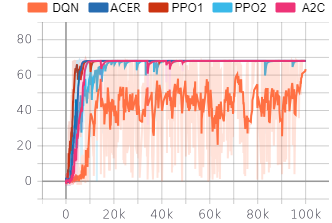
\includegraphics[width=.44\textwidth]{./images/ac_s.png}\hfill
    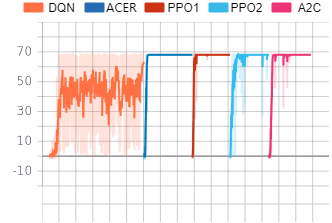
\includegraphics[width=.44\textwidth]{./images/ac_s_wall.png}
    \\[\smallskipamount]
    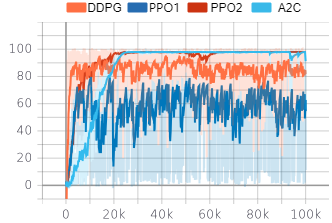
\includegraphics[width=.44\textwidth]{./images/of_s.png}\hfill
    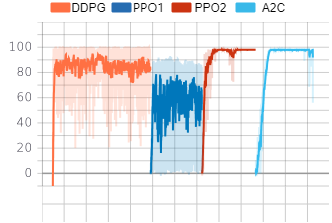
\includegraphics[width=.44\textwidth]{./images/of_s_wall.png}
    \caption{Mean reward of \textbf{Acceptance Strategy} (top left(step), top right (wall)) and of \textbf{Offer Strategy} (bottom left(step), bottom right (wall)) under single issue negotiation}
		\label{fig:single-issue}
\end{figure}

\paragraph{Evaluation} When training independent negotiator with SAOMechanism in the environment \gls{sbe}, almost all well-known \gls{drl} algorithms have the ability to learn. \gls{acer}, \gls{ppo} and A2C have learned very good acceptance strategy, the mean reward curve converged to around 70 (i.e., 68.9). However, the performance of DQN is not particularly good. For learning offer strategy, PPO2 (improved version of \gls{ppo}) and A2C perform best. The reward curve converged to around 100. The result of \gls{ddpg} are also valuable. Although the reward curve does not converge, it oscillates around a better strategy. Overall, normal version \gls{ppo} does not perform well here. 

\subsubsection{multi issues}
The training environment is almost the same as the training environment for single issue. It is based on \gls{sbe} and sets concrete limits and attributes for it, which are defined in table \ref{tab:attributes-sbe-multi-issues}.

\begin{table}[htbp]
\centering
\begin{tabular}{l l l} \toprule
\bfseries \textbf{Attributes}      & \bfseries \textbf{Value}             \\ \midrule
\textbf{Name}                    & negotiation\_env\_ac\_s, negotiation\_env\_of\_s                     \\
\textbf{Negotiation Mechanism}   & SAOMechanism                                                         \\
\textbf{Max\_Steps}              & 100                                                                  \\
\textbf{Issue}             	     & [Quantity(0, 100), Time(0, 100), Price(10, 100)]                     \\
\textbf{Competitors}             & [MyDRLNegotiator, AspirationNegotiator]                              \\
\textbf{Utility Functions}       & [LinearUtility((0, -0.25, -0.6)), LinearUtility((0, 0.25, 1))]       \\
\textbf{Actions}                 & [ACCEPT, REJCT, END, NO RESPONSE], Outcomes                                 \\
\bottomrule
\end{tabular}
\caption{Attributes of the training environment (sbe), multi-issues}
\label{tab:attributes-sbe-multi-issues}
\end{table}

In the single issue cases, the curve of mean episode reward of \textbf{multi-issues, acceptance strategy} and \textbf{multi -issues, offer strategy} are shown in \ref{fig:multi-issues}. 
\begin{figure}
    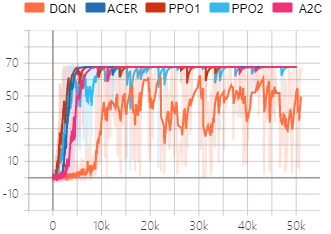
\includegraphics[width=.40\textwidth]{./images/ac_s_multi_issues.png}\hfill
    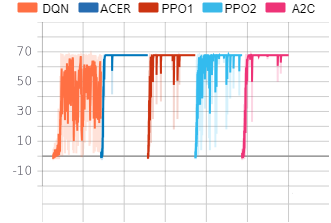
\includegraphics[width=.40\textwidth]{./images/ac_s_multi_issues_wall.png}
    \\[\smallskipamount]
    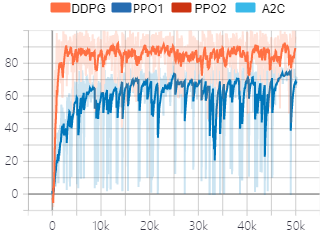
\includegraphics[width=.40\textwidth]{./images/of_s_multi_issues.png}\hfill
    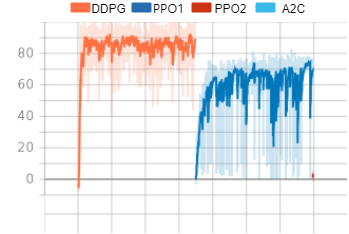
\includegraphics[width=.40\textwidth]{./images/of_s_multi_issues_wall.png}
    \caption{Mean reward of \textbf{Acceptance Strategy} (top left(step), top right (wall)) and of \textbf{Offer Strategy} (bottom left(step), bottom right (wall)) under multi-issues negotiation}
		\label{fig:multi-issues}
\end{figure}

\paragraph{Evaluation} The most characteristics of the mean episode reward curve are the same as in single-issue cases. All algoritms (DQN, ACER, PPO1, PPO2, A2C) can learn better acceptance strategy than random (best reward of around 70). It's just that the performance of DQN is not as good as others. For learning the offer strategy, DDPG and PPO2 converged to about 80 and 100, respectively. After increasing the action space, the training time increased rapidly. From the figure, we can find the curve of A2C is very strange, after 28 thousand time steps, the mean episode reward is suddenly decreasing to zero. The reason needs to be analyzed, not particularly clear.

\section{Multi-Agent Concurrent Bilateral Negotiation Environment (\gls{mcbe})} 
The agent interacting with environment have many related trainable agents (e.g. one seller, one buyer, named as trainer) as the part of learner in the model. Each seller and buyer control multiple negotiation sessions. The detail of interactive logic is shown below in \ref{fig:interacting-logic-scml}

\begin{figure}[htbp]
\centering
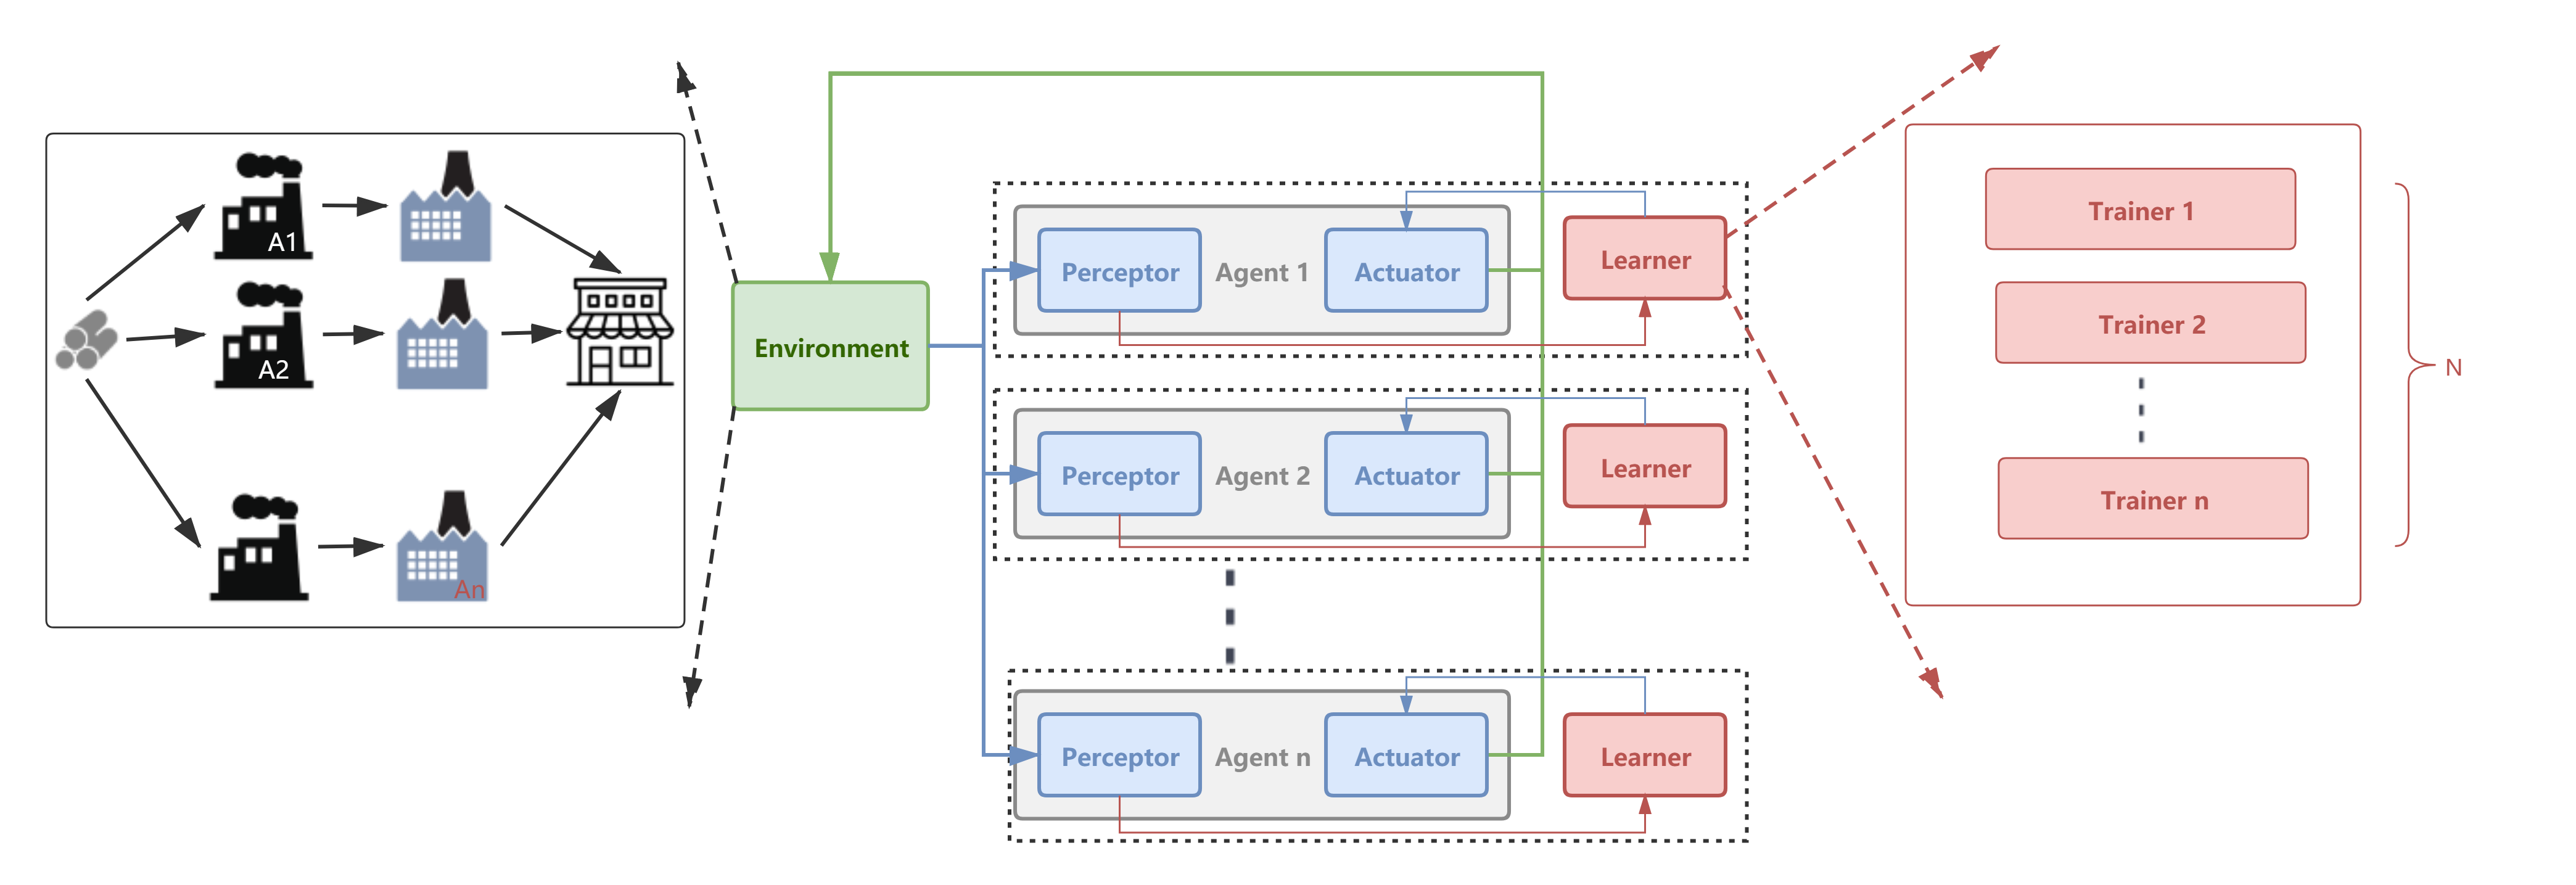
\includegraphics[width=1.0\textwidth]{./images/scnk.png}
\caption{Interactive logic based on the perspective of \gls{scml}. N: The maximum number of concurrent negotiations for a single agent}
\label{fig:interacting-logic-scml}
\end{figure}

Where environment contains six factories and two system entities (SELLER and BUYER). Three RL agents (A1, A2, An) are located at two production positions. Each RL agent contains three parts:

\begin{itemize}
\item \textbf{Perceptor} Receives state, reward from environment and send these to Learner.
\item \textbf{Actuator} Receives action from Learner and execute it in the environment.
\item \textbf{Learner} In addition to connecting with \textbf{Perceptor} and \textbf{Actuator}, it manages the multiple trainers. Because for an agent, there are many concurrent negotiation sessions. A trainer is responsible for the part of the concurrent negotiations.
\end{itemize}

Based on different algorithms, the internal components of the trainer are different. In general, the trainer will handle the training logic of concurrent negotiation. It will be introduced in the specific algorithm, diagramed in figures \ref{fig:method-maddpg-scml} and \ref{fig:method-qmix-scml}.

\subsection{In Standard SCML}
In this environment, the agent represents a factory manager.

\subsubsection{\gls{maddpg} in \gls{scml}} \label{methods:maddpg}
In the standard scml environment, one problem have to be solved by MADDPG.

\paragraph{Problem: Dynamic Range Of Negotiation Issues}At the beginning of every negotiation, the agent will determine the range which constraints values for each negotiation issue. In the experiment, the negotiation issues are \textbf{QUANTITY}, \textbf{PRICE} and \textbf{TIME}. After creating the simulated world, simulator determines the minimum and maximum values for each negotiation issue taken by the entire simulation episode, such as value of \textbf{QUANTITY} between (1, 10), \textbf{PRICE} between (0, 100) and \textbf{TIME} between (0, 100). However, for every negotiation session created inside the entire simulation episode, it has its dynamic range of negotiation issues which is determined by the agent. This question was raised based on such a situation.

From an algorithm perspective, the data flow of the model is shown in \ref{fig:method-maddpg-scml}. The basic concepts of \gls{maddpg} are introduced in chapter background \ref{background:maddpg}. Two trainers are created in MADDPG for each agent. One trainer (trainer\_seller) manages sell negotiations and another (trainer\_buyer) manages buy negotiations. 

\begin{figure}[htbp]
\centering
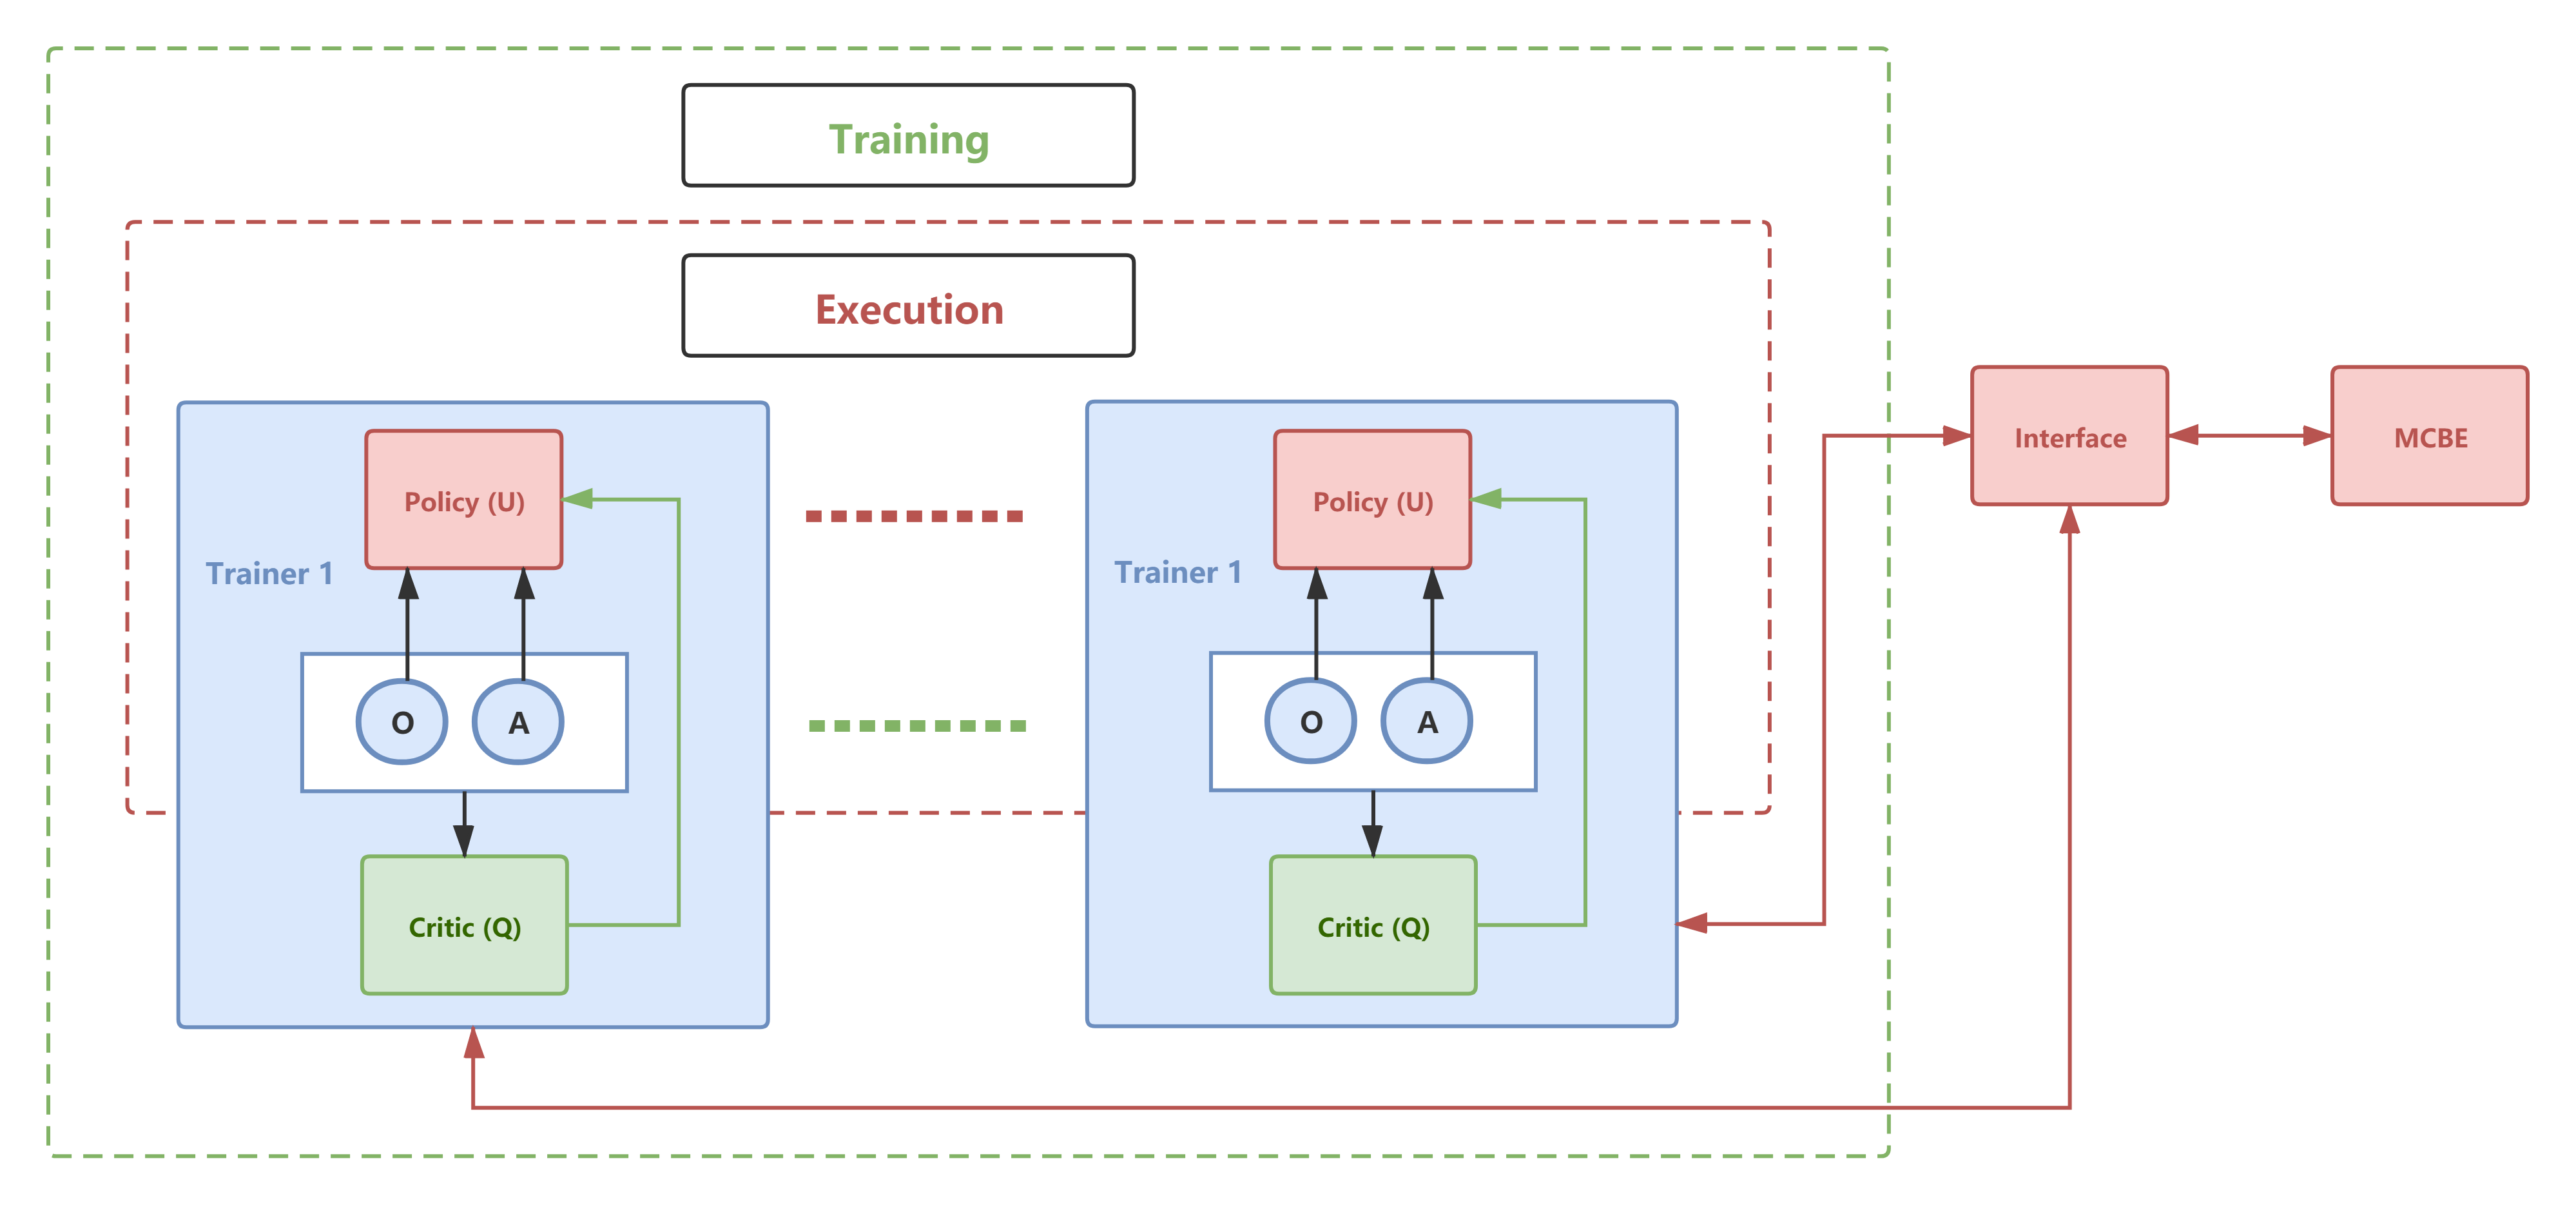
\includegraphics[width=0.80\textwidth]{./images/scml-maddpg.png}
\caption{\gls{maddpg} used in \gls{mcbe}}
\label{fig:method-maddpg-scml}
\end{figure}


In the model \ref{fig:method-maddpg-scml}, policy output action as input to related agent interacting with the environment, which outputs the observation and reward as the inputs to related trainer. Two trainers are created in the experiment:
\begin{itemize}
\item \textbf{trainer\_seller} controls all sale negotiations. The action of the trainer is the boundary value of all sale negotiation issues.
\item \textbf{trainer\_buyer} controls all buy negotiations. The action of the trainer is the boundary value of all buy negotiation issues.
\end{itemize}

The equation \ref{actions-maddpg} defines the actions of two trainers (i.e., trainer\_seller and trainer\_buyer). The observation is defined in the equation \ref{observation-maddpg}.

\begin{equation} \label{actions-maddpg}
\begin{aligned}
a_{trainer\_seller} & = \prod_{i=0}^{N_{sell}}[p_{i, l}, p_{i, r}, q_{i, l}, q_{i, r}, t_{i, l}, t_{i, r}] \\
a_{trainer\_buyer} & = \prod_{i=0}^{N_{buy}}[p_{i, l}, p_{i, r}, q_{i, l}, q_{i, r}, t_{i, l}, t_{i, r}]
\end{aligned}
\end{equation}
Where the $p_{i, l}$, $q_{i, l}$ and $t_{i, l}$ denote the left boundary value of negotiation issues (\textbf{PRICE}, \textbf{QUANTITY}, \textbf{TIME}) of agent $i$. $p_{i, r}$, $q_{i, r}$ and $t_{i, r}$ represent the right boundary value of negotiation issues of agent $i$. $N_{*}$ denotes the number of negotiations. Details of the algorithm are described in the appendix \ref{appendix:algorithms:maddpg}.  

\begin{equation} \label{observation-maddpg}
\begin{aligned}
o_{trainer\_seller} &= \prod_{i=0}^{N_{sell}}[e_{i}, m_{i}, c_{i}, n_{i, sell}, t_{i}] \\
o_{trainer\_buyer} &= \prod_{i=0}^{N_{buy}}[e_{i}, m_{i}, c_{i}, n_{i, buy}, t_{i}]
\end{aligned} 
\end{equation}

Where $e_{i}$ denotes the economic profit of agent $i$, $m_{i}$ represents the production costs, catalog prices of products are denoted by $c_{i}$. $n_{i, sell}$ and $n_{i, buy}$ represent the number of ongoing buying and selling negotiations of the agent $i$, respectively. Time is represented by $t_{i}$. 

\subsubsection{Experiment}
Standard \gls{scml} is a complex simulation world, which contains various parts with specific functions. The brief description of this simulation is introduced in chapter Background \ref{background-scml}. The experiment of this thesis focus on only the Negotiation Manager (Negotiation Control Strategy) of Decision-Maker Agent. The above mentioned method maddpg \ref{methods:maddpg} is used in this experiment. 
Scenario is diagrammed in Figure \ref{fig:scenario-standard-scml}.

\begin{figure}[htbp]
\centering
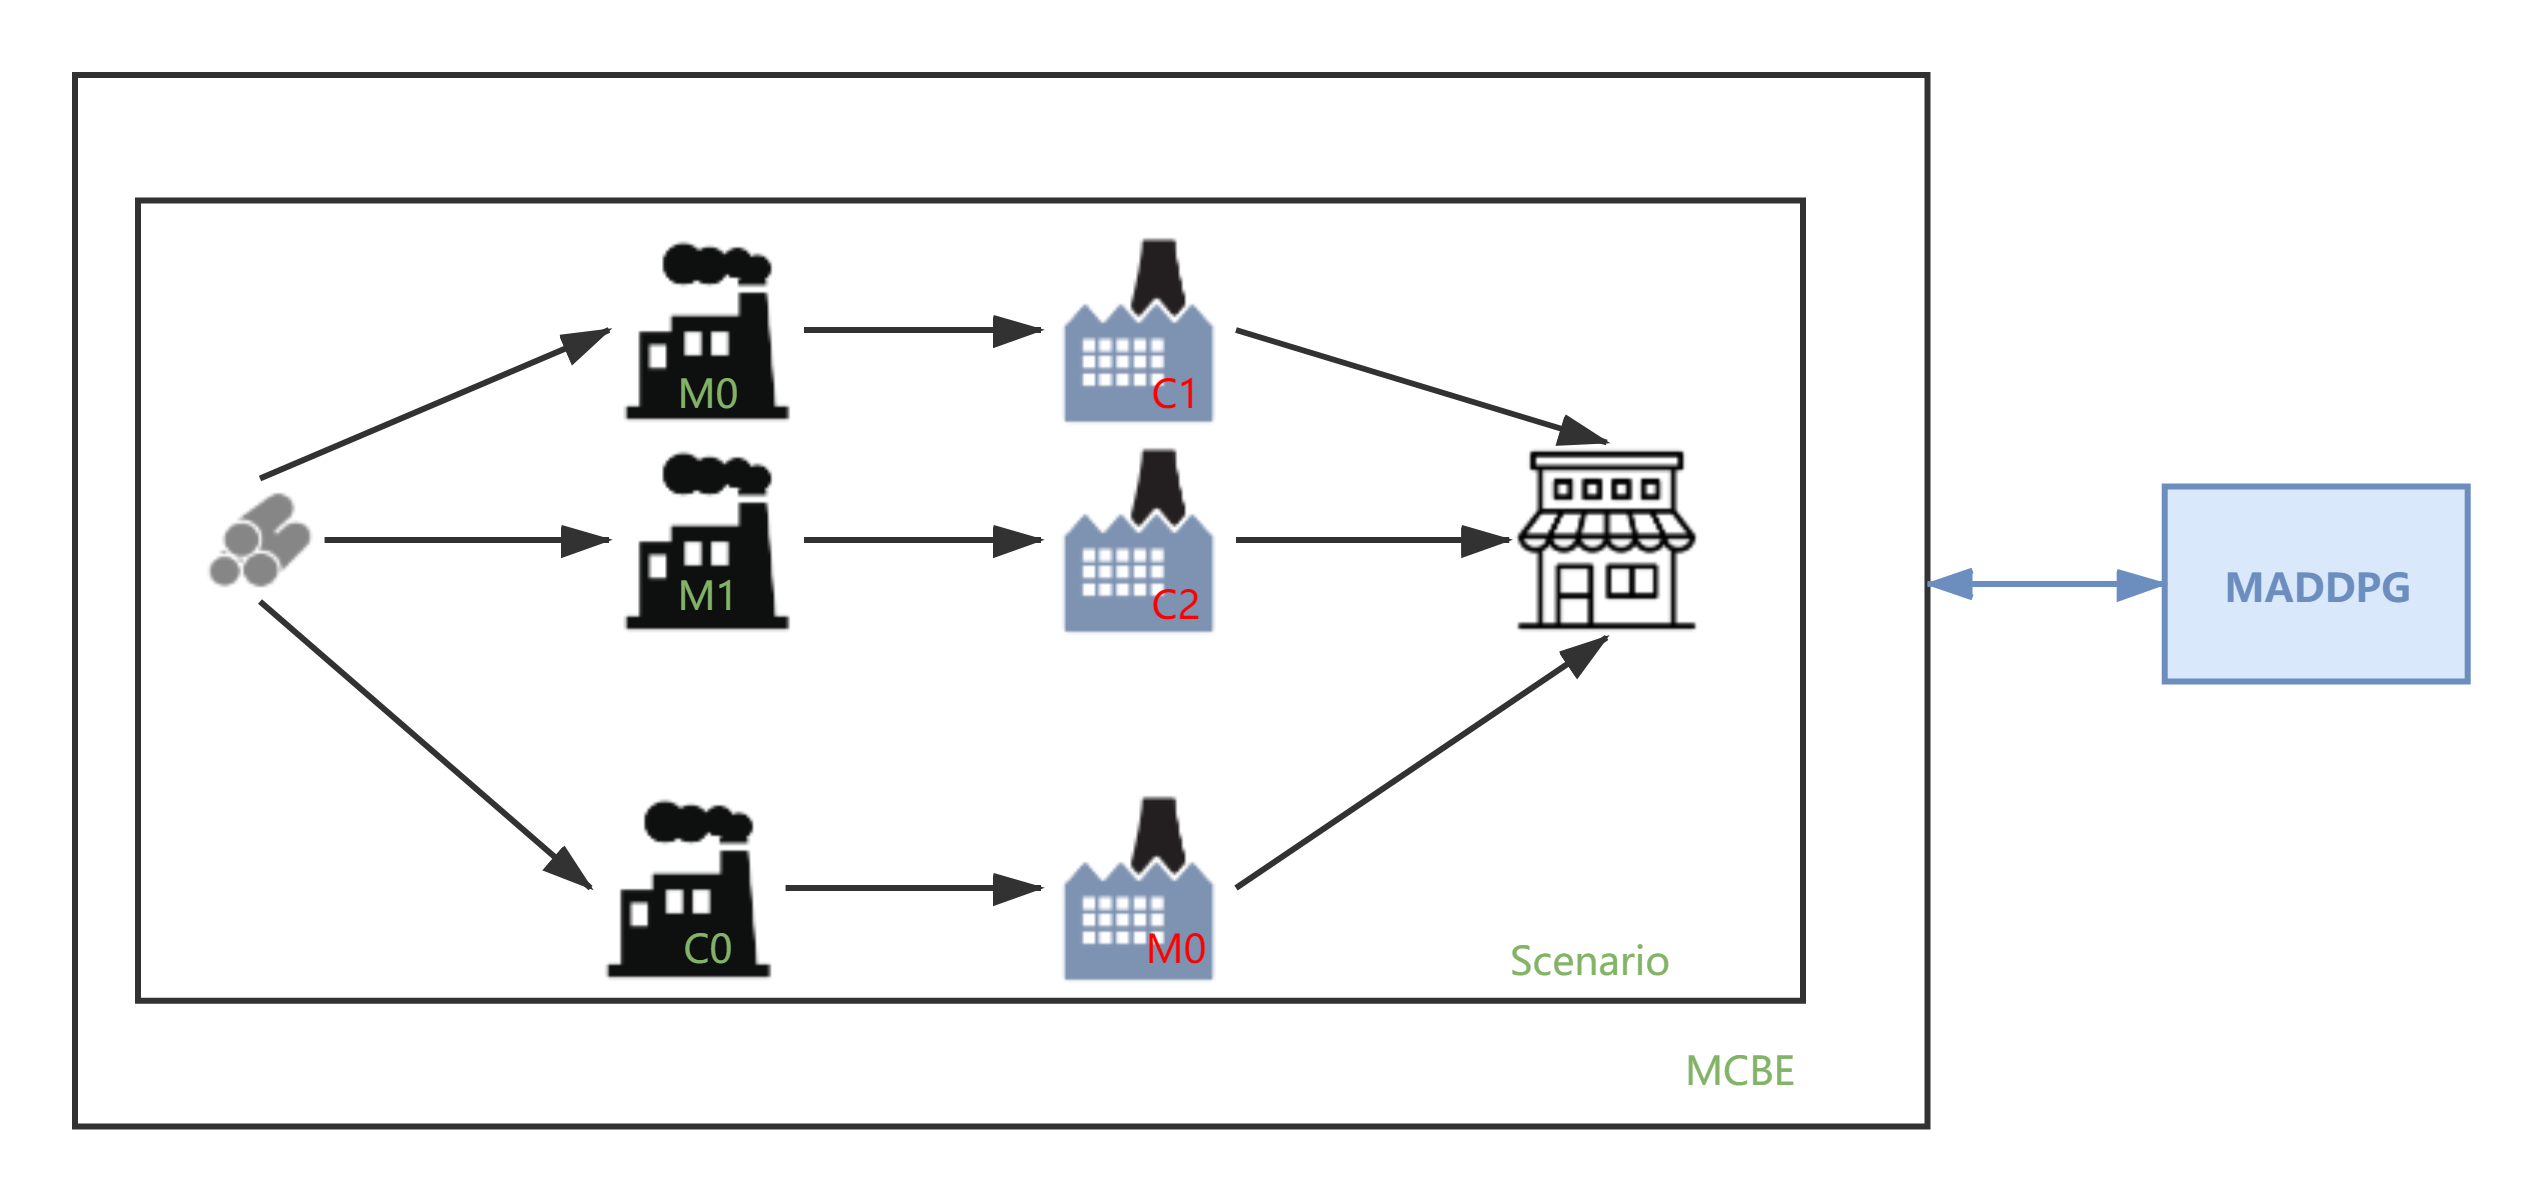
\includegraphics[width=0.80\textwidth]{./images/scenario-standard-scml.png}
\caption{M* represent My Component Based Agent with learner \gls{maddpg}, C* represent Opponent Agents, such as \gls{ind-dec-agent}}
\label{fig:scenario-standard-scml}
\end{figure}

Two different categories of agents are used for the experiments:
\paragraph{RL agents} were trained with twenty-five thousand time episodes in the training environment for the algorithms maddpg. The Rl-Agents are titled as M* in the scenario image \ref{fig:scenario-standard-scml}. All RL agents have been trained together. After training, they reload the strategy from disk and run it in the standard scml world.

\paragraph{Heuristic agent (e.g., IndDecentralizingAgent)} acts according to the strategy implemented in the scml package. The heuristic agent is named as C* in the scenario image \ref{fig:scenario-standard-scml}. There are many heuristic agents, such as IndDecentralzingAgent, BuyCheapSellExpensiveAgent, MarketAwareBuyCheapSellExpensiveAgent, etc. In this experiment, IndDecentralizingAgent is used for baseline agent.

The training environment is based on the \gls{mcbe} and sets concrete limits and attributes for it, which are defined in table \ref{tab:attributes-mcbe-dynamical-range-negotiation-issue}. The simulated world is SCML2020World designed in the package standard scml. Negotiation mechanism SAOMechanism is the default mechanism of simulated world. The environment sets the negotiation speed (negotiation rate as 1) equal to the world speed. Because the negotiation speed has a self-running speed independent of the world speed. In the default world settings, the same negotiation partner can conduct concurrent negotiations with the same partner. In this experiment, in order to fix the size of the action space, this is not allowed, which means that the maximum number of concurrent negotiations is prior knowledge. RL agents can determine the best range of negotiation issues (i.e, actions of agents). Negotiation issues are the quantity, time, and price commonly used in the SCM world.

\begin{table}[htbp]
\centering
\begin{tabular}{l l l} \toprule
\bfseries \textbf{Attributes}    & \bfseries \textbf{Value}                                             \\ \midrule
\textbf{Name}                    & scml                                                                 \\
\textbf{World}                   & SCML2020World                                                        \\
\textbf{Neogitation Mechanism}   & SAOMechanism                                                         \\
\textbf{Max Negotiation Steps}   & 10                                                                   \\
\textbf{Max Simulation Steps}    & 10                                                                   \\
\textbf{Issue}             	     & [Quantity(0, 100), Time(0, 100), Price(10, 100)]                     \\
\textbf{Competitors}             & [MyBasedAgent, DecentralizingAgent]                                  \\
\textbf{Negotiated Rate}         &    1                                                                 \\
\textbf{DNSP}                    &    True                             \\
\textbf{Actions}                 & Range of Negotiation Issues                                          \\
\bottomrule
\end{tabular}
\caption{Attributes of the training environment (mcbe), DNSP: Disallow Negotiation with Same Partners, standard scml}
\label{tab:attributes-mcbe-dynamical-range-negotiation-issue}
\end{table}

The following paragraphs will evaulate the results based on the two questions and method maddpg. 

\paragraph{Evaluation:} The results after training are shown in figure \ref{fig:dynamical-range-issues-maddpg}. From the mean episode reward curve (right in the figure \ref{fig:dynamical-range-issues-maddpg}), we can see that the agent has not learned a valuable strategy in this situation. The mean episode reward always oscillates around 7. In a sense, this is the best strategy that our RL agent can obtain. For this type of situation,  only range of negotiation issues can be controlled by the RL agents, but others part, such as offering strategy is a normal heuristic strategy.

It means, merely changing the dynamic range of negotiation issues cannot effectively improve strategy of RL agents. Compared with baseline agent IndDecentralizingAgent (left in figure \ref{fig:dynamical-range-issues-maddpg}), the score of MyComponentsBasedAgent is almost the same.  

\begin{figure}
    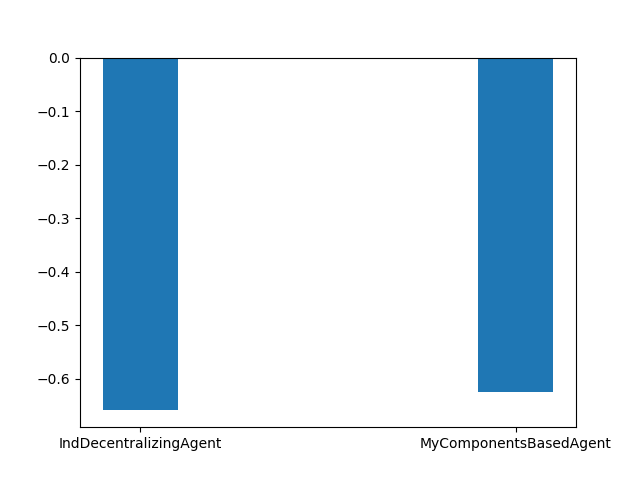
\includegraphics[width=.45\textwidth]{./images/dynamic_range_issues_maddpg.png}\hfill
    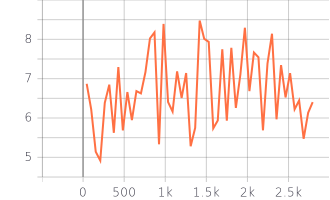
\includegraphics[width=.49\textwidth]{./images/dynamical_mean_episode_reward.png}
    \caption{Scores (left) of agents running in simulation world after training, Mean Episode Reward (right)}
		\label{fig:dynamical-range-issues-maddpg}
\end{figure}

\subsection{In SCML OneShot}
In this environment, the agent represents a factory manager.

\subsubsection{\gls{qmix} in \gls{scml-oneshot}} \label{methods:qmix-scml-oneshot}

The world created by \gls{scml-oneshot} is described in detail in the chapter background \ref{background-scml}. 

\paragraph{Question: The Offer For Every Step} Unlike in standard scml \textbf{Dynamical Range of Negotiation Issues} is not controlled by agents. Hence, question in the standard SCML does not need to be discussed here. Although the design of oneshot world is very different with the standard SCML, the key question is how to find the optimal sequence action (offer for every negotiation round). When the offer of the opponent is the same as the offer of the RL-agent's negotiator, the negotiator will accept this offer.

In the current version \gls{qmix}, which is used in the experiment, one trainable agent is create for each negotiation session. When the agents are located in different locations in the scml world, the agents have different numbers of concurrent negotiation issues. For example, since the agent \textbf{A1} shown in Figure \ref{fig:interacting-logic-scml} has three consumers, the maximum number of concurrent negotiations for it is 3. Based on this value, we need to create three trainable agents (trainers) in QMIX, and each trainable agent (trainer) controls one negotiation session of interactive agent.

The data flow is shown in fig \ref{fig:method-qmix-scml}, the total number of trainers is equal to the sum of the number of concurrent negotiations of all agents. Additionally, unlike in MADDPG, in QMIX, there is only one global learner, which can control all trainers together.

\begin{figure}[htbp]
\centering
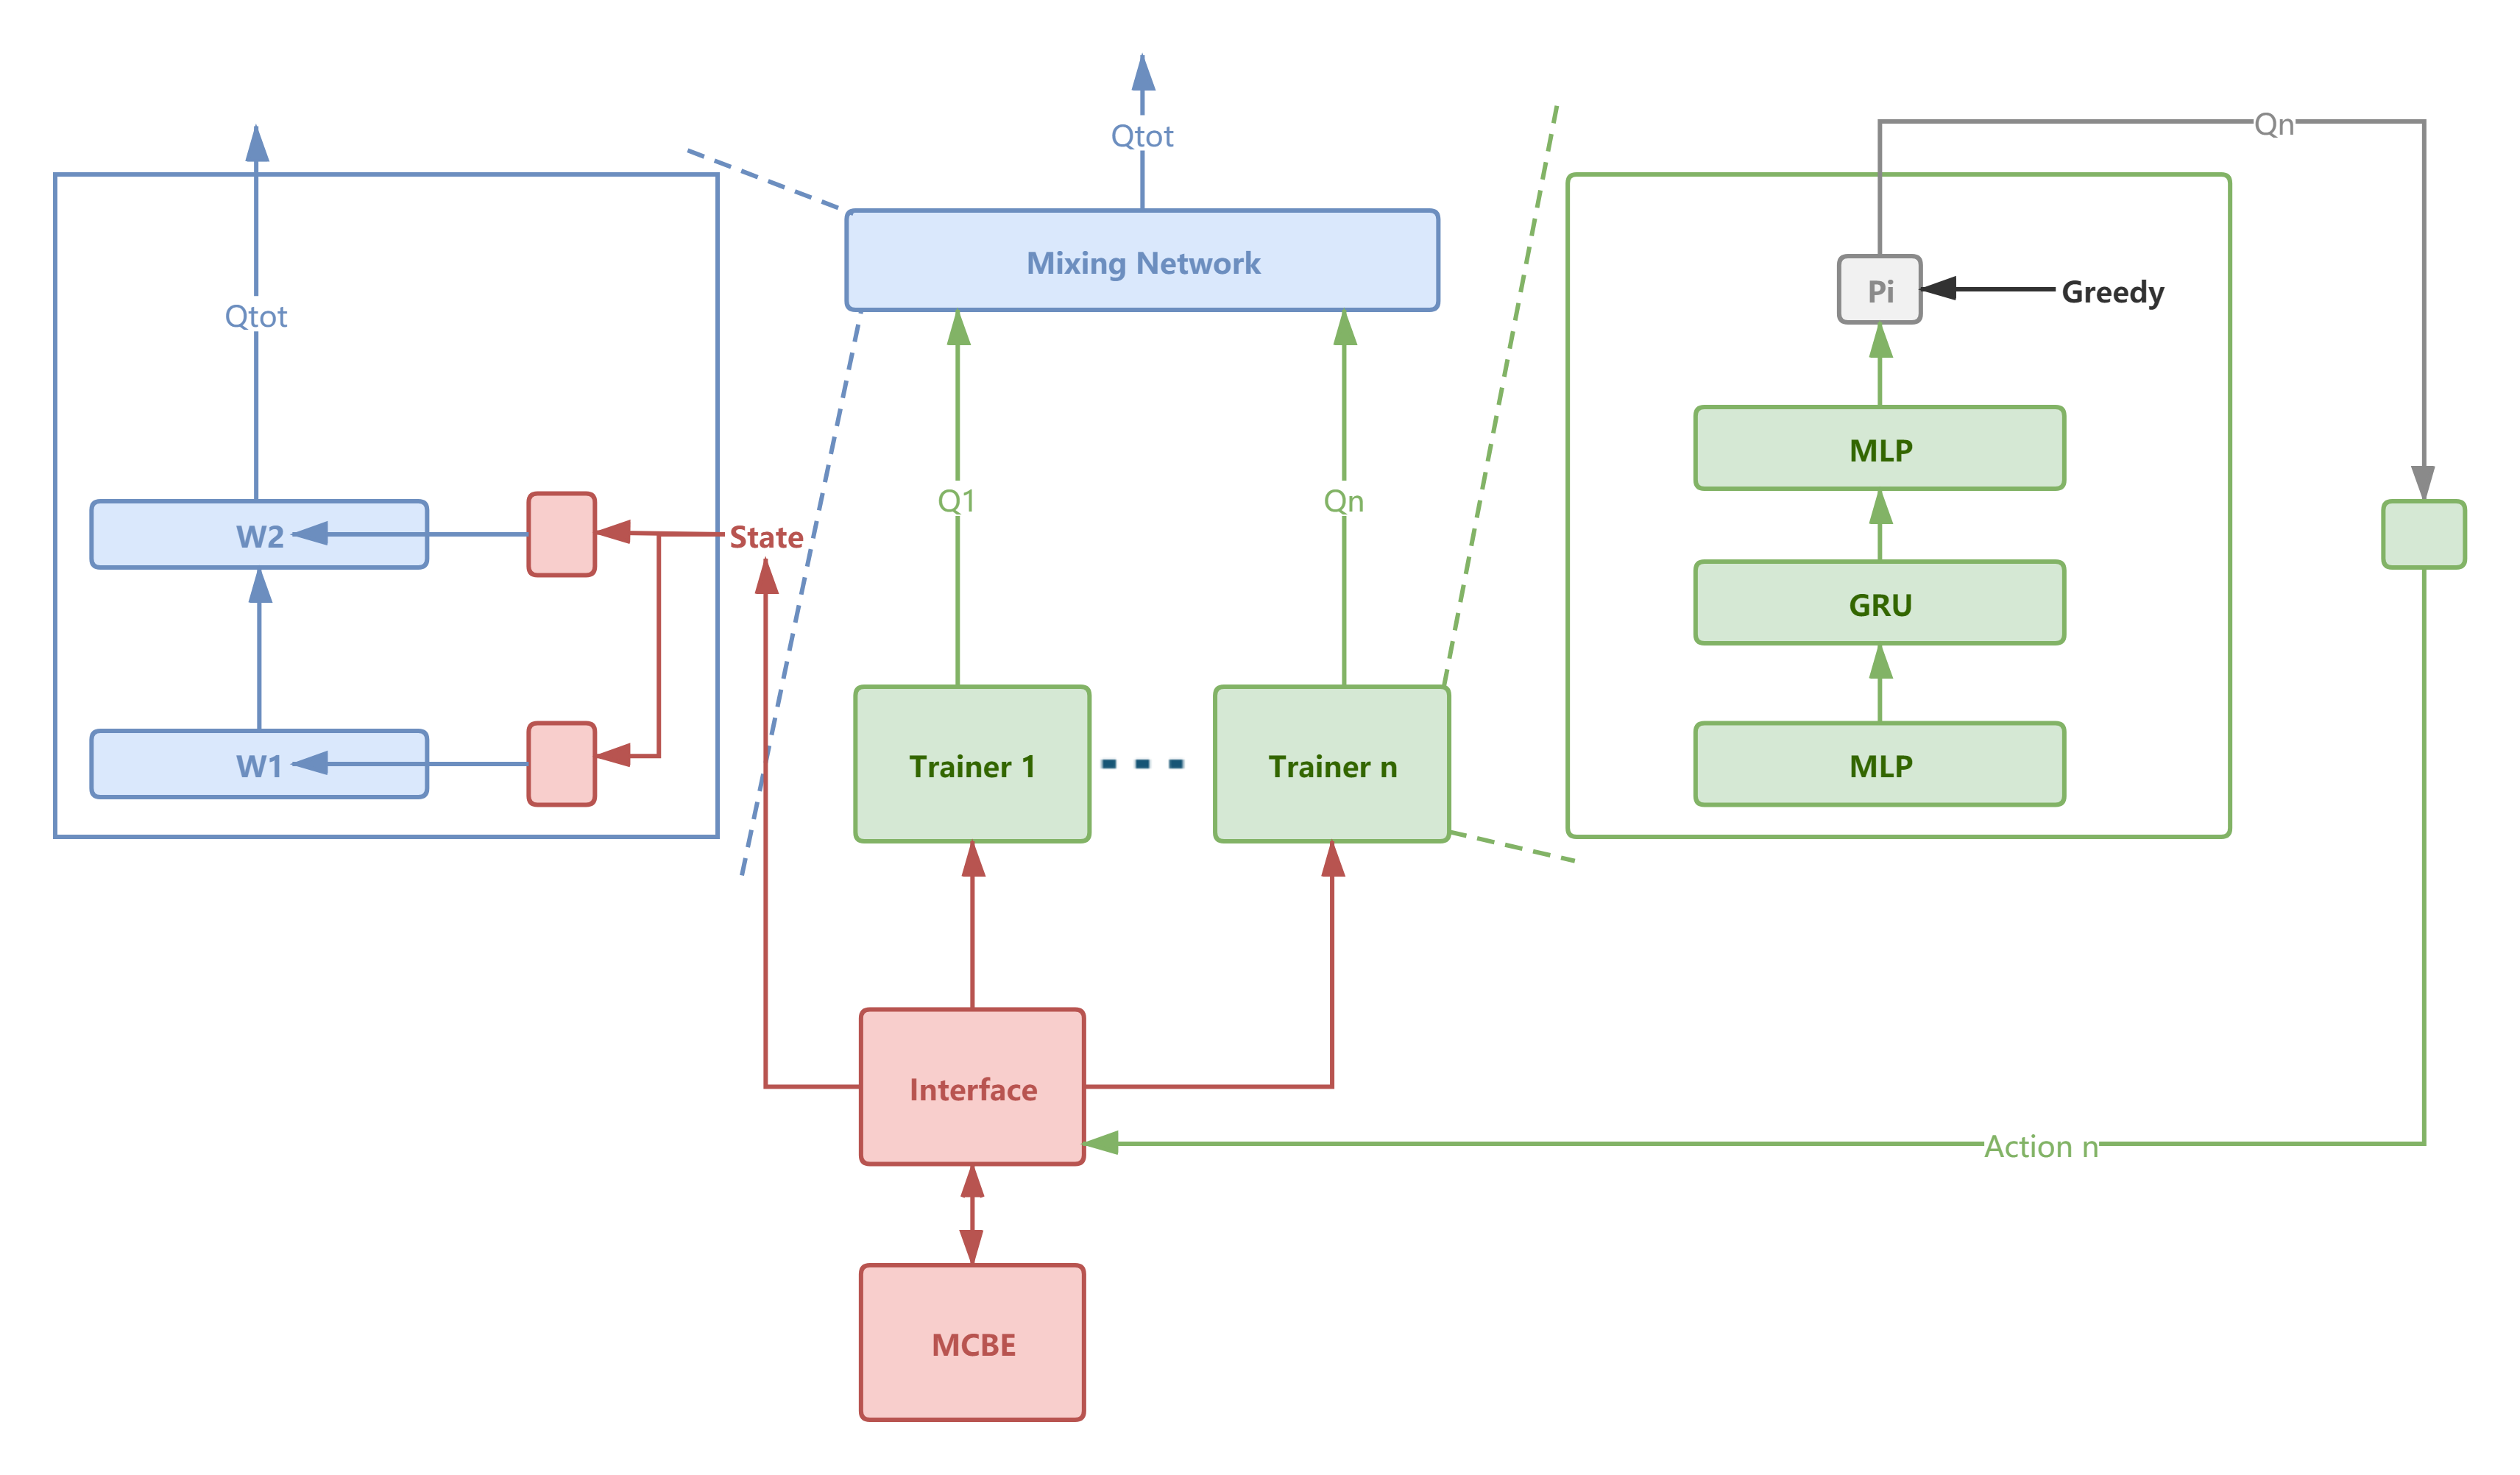
\includegraphics[width=0.80\textwidth]{./images/scml-qmix.png}
\caption{\gls{qmix} used in \gls{mcbe}}
\label{fig:method-qmix-scml}
\end{figure}

\subsubsection{Experiment}
In this experment, first, the training scenario is defined and how the various agents play is described. Secondly, the configuration of training environment is introuduced in the setting table. At the end of each experiment, the results (i.e., scores or mean episode award) will be evaluated and compared.

World created in scml-oneshot is a new simpler world which only cares about concurrent negotiation in supply chain management, and the agents used in this world can be easily transferred to standard scml. In other words, agent focus only the negotiation control strategy, which is one of the three components of a standard SCML agent\ref{background:scml2020}.
 
A brief description of this simulated world is introduced in chapter Background \ref{background-scml}. This part of the experiment only focuses on negotiation. The above mentioned method qmix \ref{methods:qmix-scml-oneshot} is used in this experiment. Two scenarios are created: \textbf{self-play} and \textbf{play-with-others}.

\paragraph{self-play}
Scenario is diagrammed in Figure \ref{fig:scenario-oneshot-scml-self-play}.
\begin{figure}[htbp]
\centering
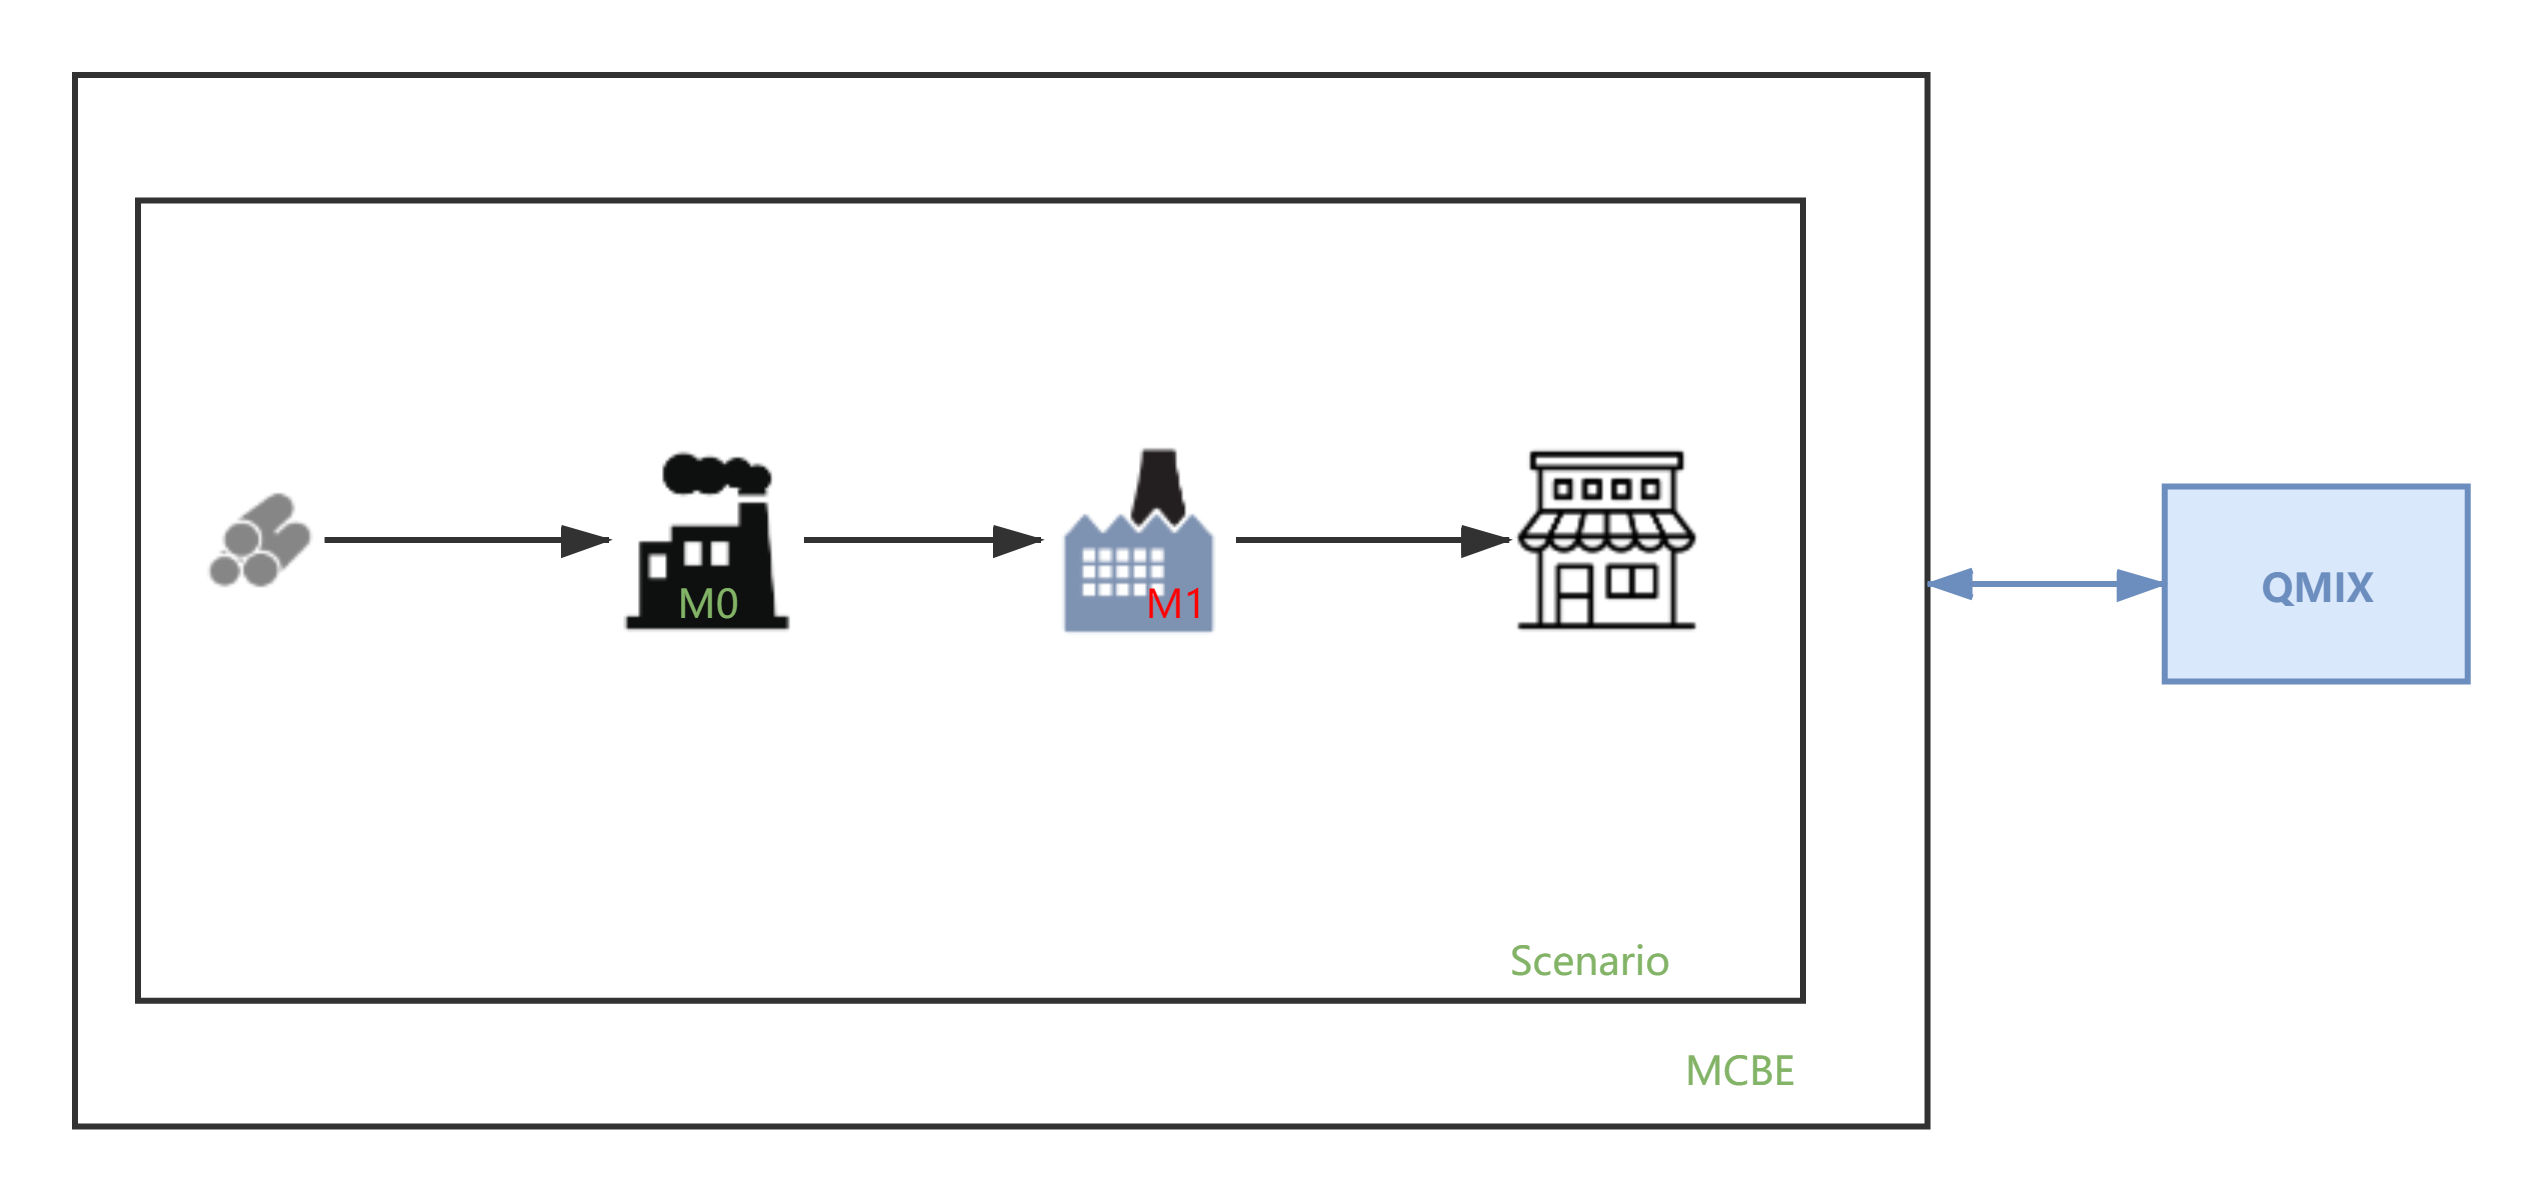
\includegraphics[width=1.0\textwidth]{./images/scenario-oneshot-scml-self-play.png}
\caption{M* represent My Component Based Agent with learner \gls{qmix}}
\label{fig:scenario-oneshot-scml-self-play}
\end{figure}

In this scenario, just only one category of agent, which is RL agent. Because it is the self-play scenario, no other heuristic agents join in.
\paragraph{RL agents} were trained with 10 thousands time steps in the training environment for QMIX. The RL-agents are named as M* in the scenario image \ref{fig:scenario-oneshot-scml-self-play}. The reward is sum of reward of each agent. Because it is a cooperative game, RL agents try to maximize profit at the end of simulation.

Although the attributes of the scml-oneshot world are very different from the standard scml world, we only consider the negotiation part. Therefore, the negotiation control attributes are almost the same, such as negotiation mechanism, max negotiation steps, max simulation steps, issues, etc.
The main difference is that we do not need to set the negotiation speed multiplier, because all negotiations will be finished inside each world (simulation) step. The name of simulated world is SCML2020OneShotWorld. The actions of each agent is outcomes (QUANTITY, PRICE) defined in the equation \ref{action-qmix}. All attributes are defined in table \ref{tab:attributes-mcbe-concurrent-negotiation-scml-oneshot}.
\begin{equation} \label{action-qmix}
a_{i} = [q_i, p_i]
\end{equation}

\begin{table}[htbp]
\centering
\begin{tabular}{l l l} \toprule
\bfseries \textbf{Attributes}    & \bfseries \textbf{Value}                                             \\ \midrule
\textbf{Name}                    & scml-oneshot-concurrent-negotiation                                  \\
\textbf{World}                   & SCML2020OneShotWorld                                                 \\
\textbf{Neogitation Mechanism}   & SAOMechanism                                                         \\
\textbf{Max Negotiation Steps}   & 20                                                                  \\
\textbf{Max Simulation Steps}    & 100                                                                   \\
\textbf{Issue}             	     & [Quantity(0, 100), Time(0, 100), Price(10, 100)]                     \\
\textbf{Competitors}             & [MyAgent, MyAgent] (self-play)                                       \\
\textbf{Actions}                 & Joint-Outcomes                                                             \\
\bottomrule
\end{tabular}
\caption{Attributes of the training environment (mcbe), scml-oneshot, self-play}
\label{tab:attributes-mcbe-concurrent-negotiation-scml-oneshot}
\end{table}

\paragraph{play with other agent} In this scenario, the opponent agent is a heuristic agent from the scml packages, such as GreedyAgent.
Scenario is diagrammed in Figure \ref{fig:scenario-oneshot-scml-play-with-greedy}.
\begin{figure}[htbp]
\centering
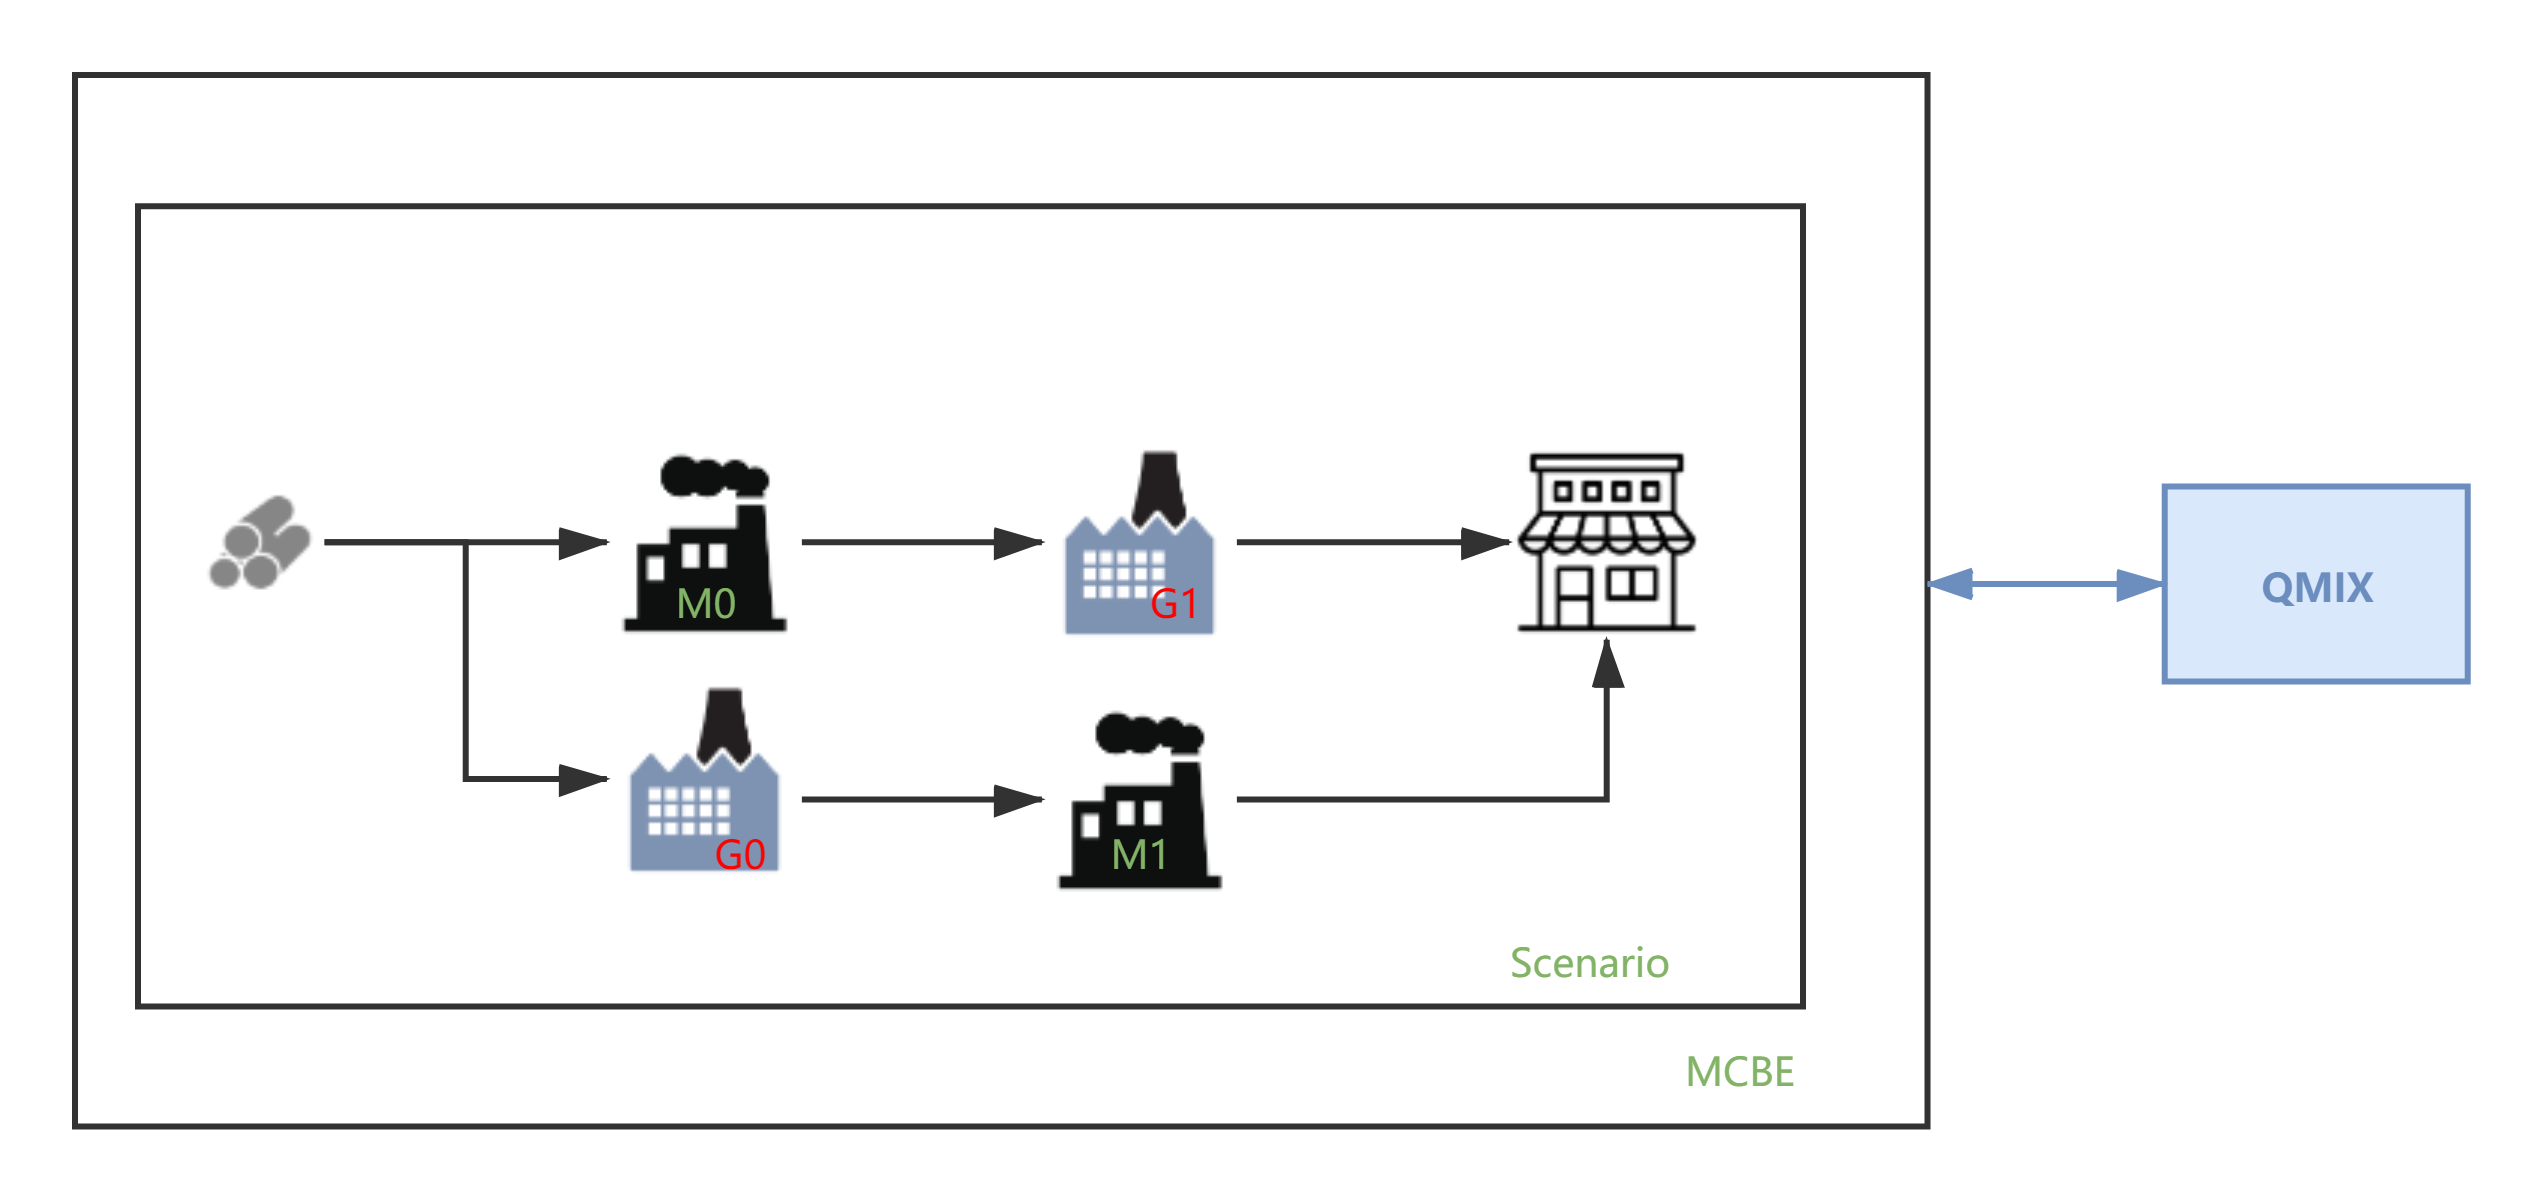
\includegraphics[width=1.0\textwidth]{./images/scenario-oneshot-scml-play-with-greedy.png}
\caption{M* represent My Component Based Agent with learner \gls{qmix}, G* represent GreedyOneShotAgent}
\label{fig:scenario-oneshot-scml-play-with-greedy}
\end{figure}

Two different categories of agents are used for the experiment:

\paragraph{RL agents} The key part is same as RL agents mentioned in self-play. In addition to the normal negotiation ability, the agent can also determine whether the negotiator is his teammate. RL agents were trained with 10 thousands time steps in the training environment with QMIX. The RL-agents are named M* in the scenario image \ref{fig:scenario-oneshot-scml-play-with-greedy}.
\paragraph{Baseline agents} There are many baseline agents realized in scml-oneshot package, such as GreedyAgent, which uses the greedy strategy to act the negotiation action. Overall, it is a simple strategy. In the future, in order to evaluate the performance of this algorithm, more sophisticated agents will need to be tested in this environment. 

The setting of this scenario is the same as in the scenario self-play. Only the competitors are changed as MyAgent vs. GreedyAgent. The negotiation mechanism is an alternative rubinstein negotiation mechanism. Negotiation issues are QUANTITY and PRICE. Based on the characteristic (all negotiations finished in each world step) of the world, time is not necessary to be considered here (i.e., set the issue time equal to the simulation step in the offer). This characteristic is briefly introduced in the section \ref{background:scml2020-oneshot}. 
All parameters are defined in table \ref{tab:attributes-mcbe-concurrent-negotiation-scml-oneshot-with-others}.

\begin{table}[htbp]
\centering
\begin{tabular}{l l l} \toprule
\bfseries \textbf{Attributes}    & \bfseries \textbf{Value}                                             \\ \midrule
\textbf{Name}                    & scml-oneshot-concurrent-negotiation                                  \\
\textbf{World}                   & SCML2020OneShotWorld                                                 \\
\textbf{Neogitation Mechanism}   & Alternative Rubinstein Mechanism                                                         \\
\textbf{Max Negotiation Steps}   & 20                                                                  \\
\textbf{Max Simulation Steps}    & 100                                                                   \\
\textbf{Issue}             	     & [Quantity(0, 100), Price(10, 100)]                     \\
\textbf{Competitors}             & [MyAgent, GreedyOneShotAgent] (play-with-others)                                       \\
\textbf{Actions}                 & Joint-Outcomes                                                             \\
\bottomrule
\end{tabular}
\caption{Attributes of the training environment (mcbe), scml-oneshot, play-with-others}
\label{tab:attributes-mcbe-concurrent-negotiation-scml-oneshot-with-others}
\end{table}

In the following paragraphs the results will be evaulate based on the two scenarios \textbf{self-paly},\textbf{ play-with-others} and method qmix raised in section \ref{methods:qmix-scml-oneshot}.

\paragraph{Evaluation of self-play} 
Curve of mean episode reward is shown in the figure \ref{fig:oneshot-self-play}. After 5 thousands time steps, the curve converges around 0. In the self-play scenario, the definition of reward is the sum reward of each agent. Therefore, while one agent gains more profits, the other agent loses more. The reward will eventually converge to a certain value, and it can be seen that the value is close to zero. The interpretation of the final convergence value will be discussed in future work. The most important question is whether this state is pareto optimal. The second question is whether RL agents can evolve on their own when the reward function is designed according to the competitive situation. This situation is very useful for training general RL agents. It means that the agent can learn more unpredictable excellent strategies through self-play.

\begin{figure}[htbp]
\centering
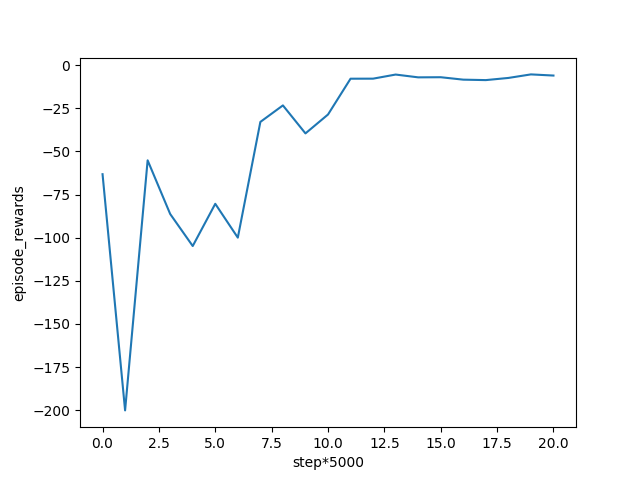
\includegraphics[width=0.55\textwidth]{./images/oneshot_self_play.png}
\caption{Mean episode reward of self-play in SCML OneShot}
\label{fig:oneshot-self-play}
\end{figure}

\paragraph{Evaluation of play-with-others}

Mean episode reward curve is shown in \ref{fig:oneshot-my-vs-greedy}. When the reward is only minus 400 at the beginning (random strategy), the reward curve finally converges to around 300. Obviously, RL agents have learned a good strategy. In addition, the training time is also very short. Thus, the results are very meaningful.

\begin{figure}[htbp]
\centering
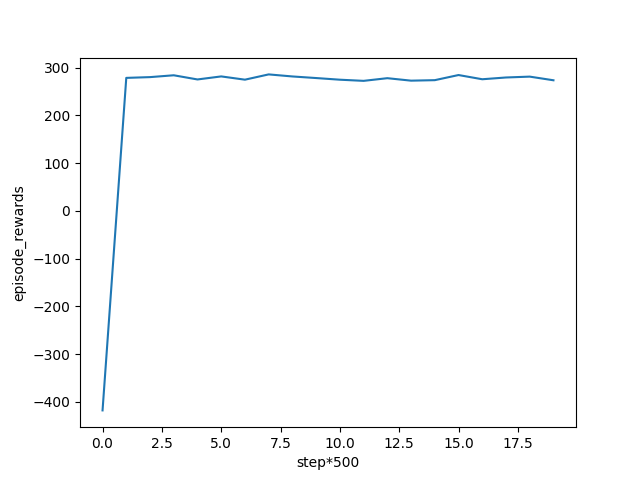
\includegraphics[width=0.55\textwidth]{./images/oneshot_my_vs_greedy.png}
\caption{Mean episode reward of my agent vs GreedyOneShotAgent under SCML OneShot}
\label{fig:oneshot-my-vs-greedy}
\end{figure}

In the scenario \textbf{self-play} and \textbf{play with other agent}, agents learned better strategy than random. It means, method \gls{qmix} is valid in scml-oneshot world.

\section{Conclusion}
The result of training of single agent (negotiator) is not bad. For multi-agent concurrent negotiations, it is not easy to implemente. The work of this thesis focuses on two algortims \gls{maddpg} and \gls{qmix}. The performance and results of \gls{qmix} have certain reference value. In the future many work and algorithms are needed to be finished and implemented in the environment \gls{mcbe}. In the future, one more experiment will be needed: In order to check the generalization ability, let trained RL agent against untrained strategy.